%%%%%%%%%%%%%%%%%%%%%%%%%%%%%%%%%%%%%%%%%%%%%%%%%%%%%

\documentclass[letterpaper, 10 pt, conference]{ieeeconf}	% Comment this line out if you need a4paper

\IEEEoverridecommandlockouts          	% This command is only needed if you want to use the \thanks command
\overrideIEEEmargins                  	% Needed to meet printer requirements.
%
\usepackage{graphics} 	% for pdf, bitmapped graphics files
\usepackage{epsfig} 	% for postscript graphics files
\usepackage{times}		% assumes new font selection scheme installed
\usepackage{amsmath} 	% assumes amsmath package installed
\usepackage{amssymb}  	% assumes amsmath package installed
\usepackage{graphicx}
\usepackage{caption}
\usepackage{subcaption}
\captionsetup{compatibility=false}
\usepackage{acronym}
\usepackage{bm}
\usepackage{cite}
\usepackage{enumerate}
\usepackage[ruled,vlined,linesnumbered]{algorithm2e}
\let\chapter\section % Necessary for List of TODOs to work. algorithm2e messes up \chapter for some reason...
\usepackage[colorinlistoftodos]{todonotes}
%\usepackage[disable]{todonotes}
\usepackage{hyperref}
%\usepackage{color}
\usepackage{gensymb}
%\usepackage{mathtools}
%
%\setlength{\textfloatsep}{\baselineskip plus 0.2\baselineskip minus 0.2\baselineskip}
%\setlength{\textfloatsep}{5pt}		% Reduces white space between floating figures and the text below them.
%
%\DeclareMathOperator{\F}{\rotatebox[origin=c]{45}{$\Box$}}
\DeclareMathOperator{\F}{\diamondsuit}
\DeclareMathOperator{\X}{\bigcirc}
\DeclareMathOperator{\G}{\Box}
\newcommand{\LTLG}{\G}
\newcommand{\LTLF}{\F}
\newcommand{\LTLX}{\X}
\newcommand{\True}{\mathtt{True}\xspace}
\newcommand{\False}{\mathtt{False}\xspace}
%
\acrodef{wrt}[w.r.t.]{with respect to}
%
% Define an "Example" environment with its own counter    
\newcounter{examplecounter}		% Example counter. Independent of theorem and other counters.
\newenvironment{myExample}
{
	\refstepcounter{examplecounter}%
	\textbf{Example \arabic{examplecounter}:}% Example #.
	\,							% Let's give our text some space.
}

% Define a "Definition" environment with its own counter    
\newcounter{definitioncounter}		% Definition counter. Independent of theorem and other counters.
\newenvironment{myDefinition}
{
	\refstepcounter{definitioncounter}%
	\textbf{Definition \arabic{definitioncounter}}%
}

% Define a "Problem" environment with its own counter    
\newcounter{problemcounter}
\newenvironment{myProblem}
{
	\refstepcounter{problemcounter}%
	\textbf{Problem \arabic{problemcounter}}% Definition #.
}

% Define an "Assumption" environment with its own counter    
\newcounter{assumptioncounter}
\newenvironment{myAssumption}
{
	\refstepcounter{assumptioncounter}%
	\textbf{Assumption \arabic{assumptioncounter}:}%
}

%
\title{\LARGE \bf
	High-level Behavior Synthesis for an ATLAS Humanoid Robot
}
\author{Spyros Maniatopoulos$^{*}$, Philipp Schillinger$^{\dagger}$, Vitchyr H. Pong$^{*}$, David C. Conner$^{\ddagger}$, and Hadas Kress-Gazit$^{*}$% 	<-this % stops a space
%\thanks{...}% <-this % stops a space
\thanks{This work was supported by DARPA / TORC Robotics \ldots}
\thanks{$^{*}$Verifiable Robotics Research Group, Sibley School of Mechanical and Aerospace Engineering, Cornell University, Ithaca, NY 14853, USA {\tt \{sm2296, vhp22, hadaskg\}\nolinkurl{@cornell.edu}}}
\thanks{$^{\dagger}$Robert Bosch GmbH, 70442 Stuttgart, Germany {\tt philipp.schillinger\nolinkurl{@de.bosch.com}}}
\thanks{$^{\ddagger}$Capable Humanitarian Robotics \& Intelligent Systems Lab, Department of Physics, Computer Science and Engineering, Christopher Newport University, Newport News, VA 23606, USA {\tt david.conner\nolinkurl{@cnu.edu}}
\todo[inline, caption = {Co-authors should review and fix contact info}]{Each author should review and fix their contact info.}}
}% end authors
%
%%%%%%%%%%%%%%%%%%%%%%%%%%%%%%%%%%%%%%%%%%%%%%%%%%%%%
%
\begin{document}
%
\maketitle
\thispagestyle{empty}
\pagestyle{empty}
%
\begin{abstract}
In this paper we \ldots
\todo[inline, caption = {Title of my TODO example (hyperlink)}]{Body of my TODO example}
\end{abstract}
%
%%%%%%%%%%%%%%%%%%%%%%%%%%%%%%%%%%%%%%%%%%%%%%%%%%%%%
\listoftodos[List of TODOs, Fixes, Open Issues]
%
%\setcounter{tocdepth}{2}
%\tableofcontents
\newpage
%%%%%%%%%%%%%%%%%%%%%%%%%%%%%%%%%%%%%%%%%%%%%%%%%%%%%
%
% --- Main sections ----
%
\section{Introduction}\label{S:intro}
% !TEX root = ../main.tex

\begin{figure}[t]
\centering
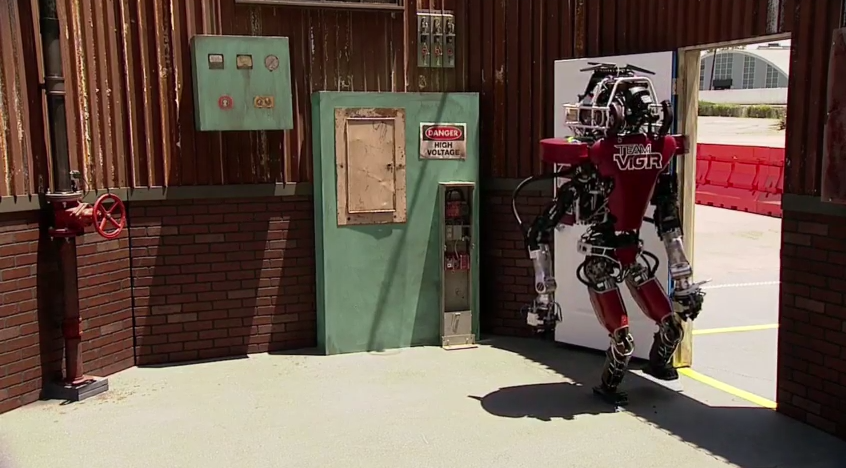
\includegraphics[width=0.99\columnwidth,clip]{./img/atlas_door_finals.png}
\caption{Team ViGIR's Atlas humanoid robot on the first day of the DRC Finals. (Photo credit: DARPA)
}
\label{Fig:AtlasDoorFinals}
\end{figure}

In preparation for the 2015 DARPA Robotics Challenge (DRC) Finals, Team ViGIR, as well as many other teams, developed an approach to high-level robot control \cite{Philipp2013Bsc, Philipp2015Msc}.
However, these approaches relied on experts developing scripted behaviors or, in the case of Team ViGIR, manually designing state machines.
In addition, there was no guarantee that the resulting high-level behavior was correct with respect to the task at hand.
Moreover, many participants observed that such approaches were fragile in practice \cite{DRC-what-happened}.

Motivated by these shortcomings, we present an approach for the automatic generation of software that implements high-level robot behaviors in a provably-correct manner.
This was enabled in part by recent advances in the field of formal methods for robotics.
Specifically, correct-by-construction mission plans can be automatically synthesized from high-level, logic-based specifications [cite ALL the papers].

\begin{myExample}\label{Ex:PickupObject}
	Consider the high-level task: ``Walk to the valve and turn it" (Fig. \ref{Fig:AtlasDoorFinals}).
	This would be an intuitive way to express the task from a non-expert user's point-of-view.
	However, \ldots (not formal, capabilities (a robot with no manipulators wouldn't be able to carry out this task), reaction to failures, etc.)
\end{myExample}

Writing a formal, logic-based specification is a non-trivial task that requires expert knowledge.
In this paper, we automatically generate the logic-based specifications from a higher level, partial, multi-paradigm specification: a description of the system's capabilities, a list of the task's goals, and the task's initial conditions.
Furthermore, most approaches in this field assume that the simple, low-level components that make up the high-level plan will work as expected, i.e., they never fail.
In this paper, we take a first step towards lifting this assumption by formally accounting for the possibility of failure when executing the low-level components.
We achieve this by generalizing the concepts of ``activation" and ``completion" as presented in \cite{Vasu2013ICRA} to deal with a different problem in logic-based synthesis.
While a failure is still a failure and there might be no way to recover, we can still achieve \emph{graceful degradation}.

Ours is an end-to-end approach that starts with an informal specification and results in an executable software implementation of a high-level plan.
We first create a discrete abstraction of the problem and automatically construct a formal task specification in a fragment of Linear Temporal Logic (\textsc{LTL}).
We then synthesize a \emph{reactive} mission plan that is guaranteed to satisfy the formal specification.
Finally, in an effort to bridge the gap between theoretical results and practice, we automatically generate a state machine that instantiates the synthesized plan in software.

In this paper, we present and experimentally validate the proposed approach in the context of a Boston Dynamics Atlas humanoid robot running the software that Team ViGIR developed for the DARPA Robotics Challenge (Fig. \ref{Fig:AtlasDoorFinals}).
However, the concepts apply to different systems.
Finally, we have implemented and open-sourced the proposed approach as a collection of Robot Operating System (ROS) packages.

\subsubsection*{Literature Survey}
\begin{itemize}
	\item Vasu's ``fast-slow" paradigm \cite{Vasu2013ICRA}
	\item Alternatives to LTL and GR(1) Synthesis
	\begin{itemize}
		\item Classic AI planners, STRIPS-type planners
		\item Optimization-based LTL synthesis (Eric Wolff)
		\item \textbf{co-safe LTL} (Lydia Kavraki, Calin Belta, etc.) We \emph{could} have used it as a different formalism and generated FlexBE state machines that way.
		\todo[inline, caption = {Comparison of GR(1) to co-safe LTL}]{Check whether co-safe LTL encodes reactivity w.r.t. adversarial environment (worst case)}
	\end{itemize}
\end{itemize}

The rest of this paper is organized as follows. \ldots

%END
%
\section{Preliminaries}\label{S:prelim}
% !TEX root = ../main.tex

\subsection{Atlas Humanoid Robot}

Atlas (Fig. \ref{Fig:AtlasDoorFinals}) is an anthropomorphic robot developed by Boston Dynamics, Inc. (BDI). 
Team ViGIR chose to leverage the basic capabilities provided by the Boston Dynamics Application Programming Interface (API).
In the context of this work, we are especially interested in BDI's ``control mode" interface (Fig. \ref{Fig:ControlModeTS}).
The active control mode dictates which joints are controlled by the low-level BDI controllers and which joints we can command.
For example, in \textsc{stand} and \textsc{manipulate} BDI's software handles balancing.

Atlas is equipped with a number of sensors, most notably a Carnegie Robotics Multisense SL\footnote{\scriptsize{\url{http://carnegierobotics.com/multisense-sl}}} mounted as the head.
For the DRC Finals, Atlas was equipped with two Robotiq 3-finger hands,\footnote{\scriptsize{\url{http://robotiq.com/products/industrial-robot-hand}}} providing basic manipulation capabilities.

\begin{figure}[t]
\centering
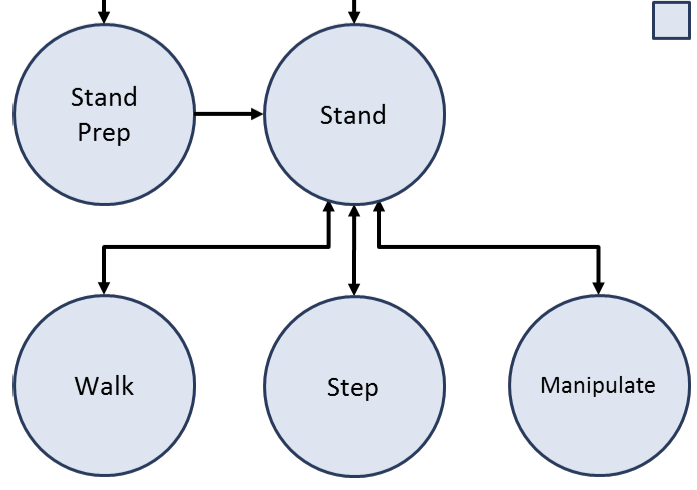
\includegraphics[width=0.99\columnwidth,clip]{./img/control_modes_ts.png}
\caption{Excerpt from the BDI control mode interface.
Some changes between modes (depicted as arrows) are unidirectional while others are bidirectional.
After Team ViGIR's initial checkout, Atlas is in the \textsc{stand\_prep} control mode.
}
\label{Fig:ControlModeTS}
%\vspace{-3 pt}
\end{figure}

\subsection{Team ViGIR's Approach to the DRC Finals}\label{S:TeamViGIR}

Team ViGIR has based its software on the Robot Operating System (ROS).
In this section, we highlight some elements of the software's design that are relevant to high-level control and behavior synthesis.
For a complete overview of Team ViGIR's approach, we refer the interested reader to \cite{TeamViGIR2014JFR}.
From this point on, we will refer to Atlas running Team ViGIR's software as the \emph{system}, $\mathcal{S}$.
\todo[inline, caption = {Replace 2014 JFR with new JFR paper}]{If the new JFR paper is accepted by February, replace this old reference, \cite{TeamViGIR2014JFR}, in the final submission.}

%\subsubsection{Major Software Components}
Since Team ViGIR uses BDI's control mode interface, some system capabilities are preconditioned on a certain control mode being active.
For example, in order to execute an arm trajectory, the system must be in the \textsc{manipulate} mode.
In addition, the system's operation has to respect the constraints on the possible control mode changes (Fig. \ref{Fig:ControlModeTS}).

In terms of manipulation, Team ViGIR employs the concept of object templates \cite{Alberto2014Humanoids}.
In brief, the system presents the human operator with perception data, e.g., a point cloud.
Then, the operator detects objects of interest and overlays an object template on top of them.
These templates contain metadata, such as relative robot poses from which the object is reachable, relative pre-grasp and grasp end-effector poses, as well as finger configurations corresponding to different grasps.
In addition, object templates provide manipulation affordances.
For instance, the ``door" template provides affordances such as ``turn (handle) clockwise" and ``push".
\todo[inline, caption = {Improve description of object templates}]{Skim Albert's paper and improve this description of OT.}

\subsubsection*{High-level Control}\label{S:FlexBE}
Team ViGIR's approach to high-level control is especially relevant to this work.
Its corner stone is the Flexible Behavior Engine\footnote{\scriptsize{\url{https://github.com/team-vigir/flexbe_behavior_engine}}} (FlexBE) \cite{Philipp2013Bsc, Philipp2015Msc}, which is a major extension of the SMACH high-level executive \cite{SMACH2010RAM}.

Using the FlexBE framework, developers create ``state implementations", $Q$. % Maybe definitions?
Each $q \in Q$ is a small, atomic block of code that interfaces with \emph{one} of the lower-level system capabilities $\mathcal{C}$.
Furthermore, each state implementation defines a number of outcomes $Out(q)$, e.g., $\{ \mathtt{done}, \mathtt{failed}, \mathtt{aborted} \}$.
The state implementations can be composed to form hierarchical state machines,\footnote{\scriptsize{\url{https://github.com/team-vigir/vigir_behaviors}}}
 which encode the logic of execution as well as the flow of data.
Specifically, state machines consist of \emph{parametrized} instantiations, $q_p \in Q_P$, of the state implementations $Q$.
For example, if a state implementation corresponds to changing control modes, its parametrized counterparts correspond to changing to specific control modes, e.g., to \textsc{stand}.
State machines also have outcomes themselves, e.g. $\{ \mathtt{finished}, \mathtt{failed} \}$.
%The top-level state machine will be referred to as a ``behavior".

Finally, both composition of state machines and supervision of their execution takes place in FlexBE's graphical user interface\footnote{\scriptsize{\url{https://github.com/team-vigir/flexbe_chrome_app}}} (GUI).
Figure \ref{Fig:FlexBESM} depicts an example of a state machine that implements a high-level behavior (opening and traversing through a door).
It was designed manually in the FlexBE GUI's editor by an expert user.

\begin{figure}[t]
\centering
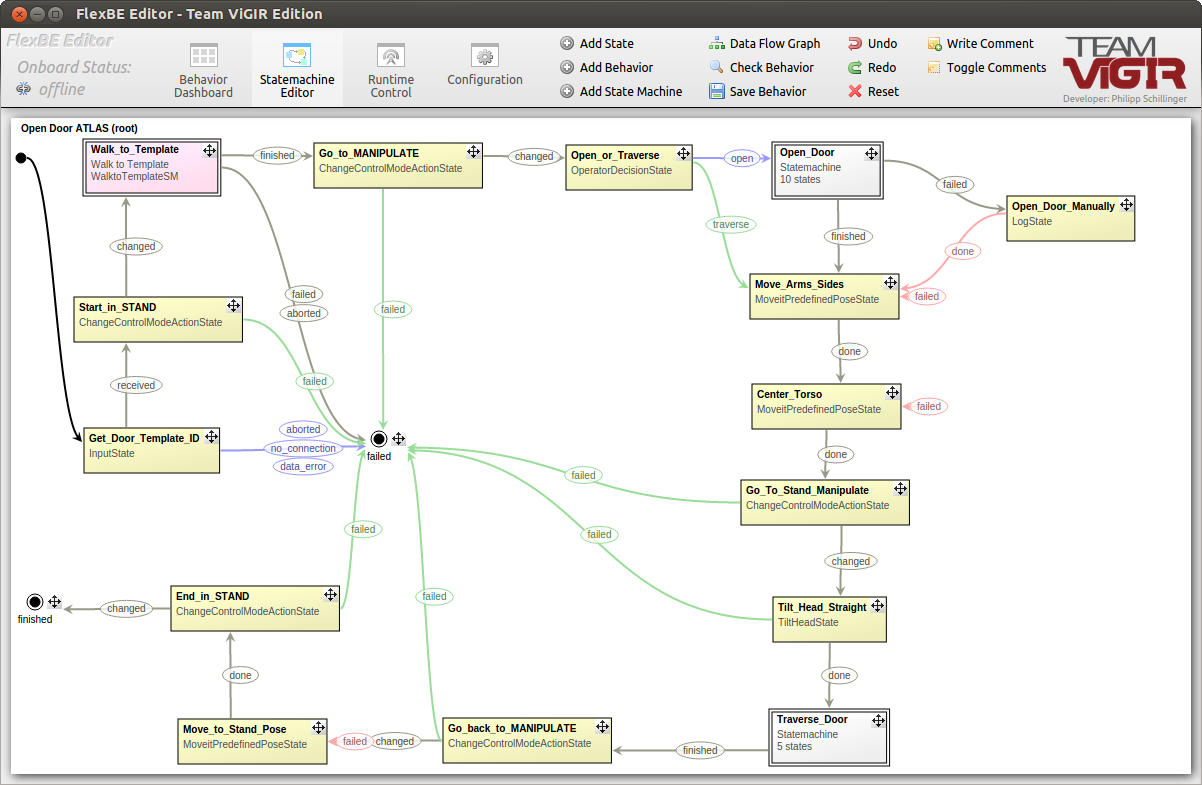
\includegraphics[width=0.99\columnwidth,clip]{./img/behavior_open_door.png}
\caption{A manually designed state machine for carrying out the DRC Finals' ``Door" task.
The initial state is indicated by the black arrow originating from the top left.
The state machine has two outcomes, ``finished" (bottom left) and ``failed" (center).
Yellow states are parametrized state implementations.
Gray and purple states are state machines.
%, and purple states are other high-level behaviors embedded in this one.
In brief, the high-level behavior implemented by this state machine is one where the system first asks the human operator to identify the door handle and then Atlas approaches the door, turns the handle, and steps through the door.
}
\label{Fig:FlexBESM}
\end{figure}

\subsection{Linear Temporal Logic and Reactive LTL Synthesis}\label{S:GR1}

Linear Temporal Logic (\textsc{ltl}) is a formal language that combines Boolean ($\lnot$, $\wedge$, $\lor$) and temporal (next $\LTLX$, until $\mathcal{U}$) operators.
Additional temporal operators, always $\LTLG$, eventually $\LTLF$, can be derived from those.
\textsc{LTL} formulas are constructed from Boolean atomic propositions $\pi \in AP$.
In the context of our work, the set of atomic propositions, $AP$, consists of propositions controlled by the system, $\mathcal{Y}$, and propositions controlled by the dynamic, and possibly adversarial, environment, $\mathcal{X}$. That is, $AP = \mathcal{X} \cup \mathcal{Y}$.

In order to synthesize \emph{reactive} mission plans in a computationally tractable manner, we use the \textsc{gr(1)} fragment of \textsc{ltl} \cite{Bloem2012GR1}.
\textsc{GR(1)} formulas $\varphi$ have an assume-guarantee structure between the dynamic environment ($e$) and the system ($s$):
%$\varphi = (\varphi_e \Rightarrow \varphi_s)$, where:
%$$\varphi_e = \varphi_e^i \wedge \varphi_e^t \wedge \varphi_e^g, \; \varphi_s = \varphi_s^i \wedge \varphi_s^t \wedge \varphi_s^g,$$
\begin{equation}\label{GR1Formula}
\begin{split}
	\varphi &= (\varphi_e \Rightarrow \varphi_s),\\
	\varphi_e &= \varphi_e^i \wedge \varphi_e^t \wedge \varphi_e^g,\\
	\varphi_s &= \varphi_s^i \wedge \varphi_s^t \wedge \varphi_s^g,
\end{split}
\end{equation}
where the superscript $i$ denotes initial conditions, $t$ safety assumptions/requirements, and $g$ liveness assumptions/requirements (i.e., goals) for $e$ and $s$, respectively. 

\textsc{GR(1)} synthesis involves setting up a two-player game between $e$ and $s$ \cite{Bloem2012GR1}.
If a \textsc{gr(1)} specification $\varphi$ is realizable for $s$, we can extract a finite-state automaton; specifically, a Mealy machine. 
This automaton encodes a strategy for $s$ that guarantees $\varphi_s$ for any evolution of $e$ that satisfies $\varphi_e$.
\todo[inline, caption = {If enough space, define Mealy machine}]{If there's any space left, define the FSA/Mealy machine mathematically. Possibly connect to FlexBE SMs later.}

% END
%
\section{Problem Statement}\label{S:problem}
% !TEX root = ../main.tex

\begin{myProblem}\label{OverarchingProblem}
\textbf{(High-level Behavior Synthesis):}
	Given a system $\mathcal{S}$, which comprises a robot and its primitive capabilities $\mathcal{C}$, a desired reaction to failures $\mathcal{F}$ specified by the system designer, and a task $\mathcal{T}$ specified by a non-expert user, in terms of its goals $\mathcal{G}$ and initial conditions\footnote{If the task specification process is taking place online, i.e., during system operation, then the initial conditions could also be detected automatically.}
	 $\mathcal{I}$, automatically generate the software implementation of a high-level mission plan that \emph{guarantees} the system will either:
	\begin{enumerate}[i]
		\item achieve the goals $\mathcal{G}$ safely, if possible,
		\item or react according to the specification $\mathcal{F}$, if the execution of any primitive capabilities $\mathcal{C}$ does not succeed.
	\end{enumerate}
\end{myProblem}

Problem \ref{OverarchingProblem} involves three main considerations.
First, we have to accept input, $\mathcal{T}$, from non-expert users.
In addition, we have to formally specify the task to be carried out by the system in order to capture the goals and initial conditions, system-specific safety requirements, and the possibility of failure.
This formal specification should also account for the desired system's reaction to failure $\mathcal{F}$.
Finally, we want to automatically generate a high-level plan that is verifiably correct with respect to the formal specification, as well as its software implementation.
These considerations give rise to the following subproblem statements, which together outline our approach to tackling Problem \ref{OverarchingProblem}.

\begin{myProblem}\label{DiscreteAbstractionProblem}
\textbf{(Discrete Abstraction):}
%Given Atlas' control mode transition constraints and the available actions $\mathcal{A}$, 
Define a discrete abstraction $\mathcal{D}$ of a robot-plus-software system, $\mathcal{S}$, that captures both the execution and possible outcomes of its primitive capabilities $\mathcal{C}$.
In addition, maintain a mapping, $\gamma: \mathcal{D} \rightarrow \mathcal{C}$, which grounds\footnote{We refer the reader to \cite{Grounding2013} for a review of symbol grounding in robotics.}
 the abstract symbols of this discrete abstraction to the primitive capabilities $\mathcal{C}$ of the system $\mathcal{S}$.
\end{myProblem}

\begin{myProblem}\label{SpecificationProblem}
\textbf{(Formal Task Specification):}
Given a task $\mathcal{T}$ in terms of goals $\mathcal{G} = \{ g_1, g_2, \ldots, g_n \}$ and initial conditions $\mathcal{I} = \{ i_1, i_2, \ldots, i_m \}$,
a desired reaction to failures $\mathcal{F}$,
and the discrete abstraction $\mathcal{D}$ of the system $\mathcal{S}$ that is to carry out the task,\footnote{In general, a discrete abstraction of the robot's workspace would also be an input to this problem. However, we are not modeling it explicitly here.}
 automatically generate a specification $\mathcal{T}_\mathcal{S}$ that encodes, in a formal language, the task being carried out by $\mathcal{S}$ while reacting to failures according to $\mathcal{F}$.
\end{myProblem}

To illustrate these concepts, we revisit Example \ref{Ex:TurnValve}. 
The system $\mathcal{S}$ is Atlas running Team ViGIR's software.
We could say that the task's goals $\mathcal{G}$ are $\{ \mathtt{turn\_valve} \}$ and its initial conditions $\mathcal{I}$ are, e.g., $\{ \mathtt{stand} \}$.
Its primitive capabilities $\mathcal{C}$ include walking, rotating the wrist joint, and closing the fingers.
The system-specific safety requirements (e.g., action preconditions and control mode changes) are encoded in $\mathcal{D}$.

\begin{myProblem}\label{BehaviorSynthesisProblem}
\textbf{(Mission Plan \& Software Implementation):}
%\textbf{(Synthesis):}
Given a formal task specification $\mathcal{T}_\mathcal{S}$, synthesize a reactive mission plan that is guaranteed to satisfy $\mathcal{T}_\mathcal{S}$, if one exists.
Additionally, if such a plan exists, and given the mapping $\gamma$, automatically generate a software implementation of the reactive mission plan. 
\end{myProblem}

We present our approach in Sections \ref{S:abstraction}, \ref{S:ltl}, and \ref{S:synthesis}.

% END
%
\section{Discrete Abstraction}\label{S:abstraction}
% !TEX root = ../main.tex

\subsection{Control Modes \& Actions}

We model ATLAS' control mode interface (c.f. Fig. \ref{Fig:ControlModeTS}) as a transition system $(\mathcal{M}, \boldsymbol\rightarrow)$, where $\mathcal{M}$ is the set of states, each corresponding to one control mode, $m \in \mathcal{M}$, and $\boldsymbol\rightarrow$ is a set of valid control mode transitions (subset of $\mathcal{M} \times \mathcal{M}$).
In addition, we define $Adj(m) = \{ m^\prime \in \mathcal{M} \; | \; (m, m^\prime) \in \; \boldsymbol\rightarrow \}$ and also allow self-transitions, i.e., $m \in Adj(m), \; \forall m \in \mathcal{M}$.

ATLAS can perform actions. Each action, $a \in \mathcal{A}$, is considered discrete and it corresponds to a software component, e.g., generation of a footstep plan or closing the robot's fingers.
Actions may also have one or more preconditions.
Action preconditions can be control modes or other actions, i.e., $Prec(a) \in 2^{(\mathcal{A} \cup \mathcal{M})}$, $a \not \in Prec(a)$, $\forall a \in \mathcal{A}$.

\subsection{Atomic Propositions}

\todo[inline, caption = {Activation--Outcomes or just Completion-Failure ?}]{Write LTL formulas in terms of any possible outcome, $o \in Out(a)$, or only of completion and failure, $\{c, f\}$?}

We adopt a paradigm that generalizes the one in \cite{Vasu2013ICRA}.
We abstract the discrete actions, $a \in \mathcal{A}$, that ATLAS can perform using one system proposition, $\pi_a$, per action and one environment proposition, $\pi_a^o$, per possible outcome of that action, $o \in Out(a)$.
Similarly,\footnote{The distinction between action and control mode propositions is purely for the sake of clarity of notation. There is nothing special about either.}
for each control mode, $m \in \mathcal{M}$, we have a system proposition $\pi_m$ and a number of outcome propositions $\pi_m^o$.
For both actions and control mode transitions, the outcomes that are of most interest in the context of this paper are completion ($c$) and failure ($f$) of the action. That is, $Out(a) = Out(m) = \{ c, f \}$
Therefore, the set of atomic propositions $AP$ is given by Eq. \eqref{ActOutAP}:

\begin{subequations}
	\label{ActOutAP}
	\begin{align}
		\mathcal{Y} &= \bigcup \limits_{a \in \mathcal{A}} \pi_a \bigcup \limits_{m \in \mathcal{M}} \pi_m,\\
		\mathcal{X}^\prime &= \mathcal{X} \bigcup \limits_{a \in \mathcal{A}} \bigcup \limits_{o \in Out(a)} \pi_a^o \bigcup \limits_{m \in \mathcal{M}} \bigcup \limits_{o \in Out(m)} \pi_m^o,
	\end{align}
\end{subequations}
where $\mathcal{X}$ are environment propositions other than outcome propositions, e.g., ones that abstract sensors, as per \cite{KGFP_TRO09}.

% END
%
\section{Formal Task Specification}\label{S:ltl}
% !TEX root = ../main.tex

\subsection{Multi-Paradigm Specification}\label{S:multi-paradigm}

Specifying a robot task in a formal language can be a time consuming and error prone process.
It also requires an expert user.
%, unless a natural language based approach is used \cite{Lignos2015AURO}. 
To alleviate these issues, we employ a multi-paradigm specification approach. 
We first observe that there are portions of the task specification $\mathcal{T}_\mathcal{S}$ that are going to be system-specific and portions that are going to be task-specific, such as the task's goals.
Intuitively, a non-expert user should only have to specify the goals $\mathcal{G}$ without worrying about the internals of the robot and the software it is running.
We can infer which actions $\mathcal{A}$ are pertinent to a task and use the discrete abstraction $\mathcal{D}$ as the basis for automatically generating the portion of the formal specification that is related to the system itself.
Finally, the initial conditions $\mathcal{I}$ are either specified by the user or detected at runtime.

Thus, referring to Problem \ref{SpecificationProblem}, we get the goals $\mathcal{G}$ and initial conditions $\mathcal{I}$ from a user.
The discrete abstraction $\mathcal{D}$ is system-specific and has been defined \emph{a priori} by the expert system designers, according to Section \ref{S:abstraction}.
We can now automatically generate the task specification $\mathcal{T}_\mathcal{S}$ in (the \textsc{gr(1)} fragment \cite{Bloem2012GR1} of) Linear Temporal Logic.
Since \textsc{ltl} is compositional, we can generate individual formulas and then conjunct them to get the full \textsc{ltl} specification.


\subsection{Specification of Actions and Control Mode Constraints}

Since the activation of capabilities is controlled by the system, the corresponding \textsc{ltl} formulas will be in $\varphi_s$, the safety requirements (see Section \ref{S:GR1}).
Conversely, we do not control the outcome of activation; the adversarial environment does.
Therefore, the \textsc{ltl} formulas specifying the behavior of outcomes will be in $\varphi_e$, the safety assumptions.

\subsubsection{General Formulas}

We say that an activation proposition $\pi_y$, $y \in \{a, m\}$, is $\True$ when the corresponding primitive capability is being activated and $\False$ when it is not being activated\footnote{Note that this is in contrast to the work of Raman, et al. \cite{Vasu2013ICRA}, where, e.g., $\pi_{camera}$ being $\False$ stands for the act of \emph{deactivating} the corresponding primitive capability, i.e., turning a camera off.}.
Therefore, the system safety requirement \eqref{PropositionDeactivationFormula} dictates that all activation propositions $\pi_y \in \mathcal{Y}$ should turn $\False$ once an outcome has been returned.
Note that the left-hand side of formula \eqref{PropositionDeactivationFormula} is only $\True$ at those distinct time steps where an outcome was just returned.

\begin{equation}\label{PropositionDeactivationFormula}
	\bigwedge \limits_{o \in Out(y)} \LTLG \Big( \pi_y \wedge \LTLX \pi_y^o \Rightarrow \LTLX \lnot \pi_y \Big)
\end{equation}

The environment safety assumption \eqref{OutcomeMutexFormula} dictates that the outcomes, $\pi_y^o$, of the activation of any system capability are mutually exclusive (e.g., an action cannot both succeed and fail).
Formula \eqref{OutcomeMutexFormula} also allows for no outcome being $\True$.

\begin{equation}\label{OutcomeMutexFormula}
	\bigwedge \limits_{o \in Out(y)} \LTLG \Big( \LTLX \pi_y^o \Rightarrow \bigwedge \limits_{o^\prime \neq o} \LTLX \lnot \pi_y^{o^\prime} \Big)
\end{equation}

The environment safety assumption \eqref{ActionOutcomeConstraintFormula} constraints the value of outcomes.
Specifically, it dictates that, if an outcome is $\False$ and the corresponding capability is not being activated, then that outcome should remain $\False$.
It is a generalization of formula (4) in \cite{Vasu2013ICRA}.

\begin{equation}\label{ActionOutcomeConstraintFormula}
	\bigwedge \limits_{o \in Out(y)} \LTLG \Big( \lnot \pi_y^o \wedge \lnot \pi_y \Rightarrow \LTLX \lnot \pi_y^o \Big)
\end{equation}

%%%%%%%%%%%%%%%%%%%%%%%%%%%%%%%%%%%%%%%%%%%%%%%%%%%%%

\subsubsection{Action-specific Formulas}

The following formulas encode the connection between the activation and the possible outcomes of the robot's actions, $a \in \mathcal{A}$.

%The environment safety assumptions \eqref{ActionOutcomeConstraintFormula} govern the value of outcomes in the next time step. 
%%Specifically, formula \eqref{ActionOutcomeConstraintsFormula3} says that if an outcome has been returned, and the corresponding action is re-activated, then any outcome can become $\True$. 
%Specifically, formula \eqref{ActionOutcomeConstraintFormula} dictates that, if an outcome is $\False$ and the corresponding action is not activated, then that outcome should remain $\False$.
%%This pair of formulas is a generalization of the ``fast-slow" formulas (3) and (4) in \cite{Vasu2013ICRA}.
%It is a generalization of formula (4) in \cite{Vasu2013ICRA}.

%\begin{subequations}
%	\label{ActionOutcomeConstraintsFormula}
%	\begin{align}
%		\LTLG& \Big( \bigvee \pi_a^o \wedge \pi_a \Rightarrow \bigvee \LTLX \pi_a^o \Big)\label{ActionOutcomeConstraintsFormula3}\\
%		\bigwedge \limits_{o \in Out(a)} \LTLG& \Big( \lnot \pi_a^o \wedge \lnot \pi_a \Rightarrow \LTLX \lnot \pi_a^o \Big)\label{ActionOutcomeConstraintsFormula4}
%	\end{align}
%\end{subequations}

%\begin{equation}\label{ActionOutcomeConstraintFormula}
%	\bigwedge \limits_{o \in Out(a)} \LTLG \Big( \lnot \pi_a^o \wedge \lnot \pi_a \Rightarrow \LTLX \lnot \pi_a^o \Big)
%\end{equation}

The environment safety assumption \eqref{ActionOutcomePersistenceFormula} dictates that the value of an outcome should not change if the corresponding action has not been activated again. 
In other words, outcomes persist through time.

\begin{equation}\label{ActionOutcomePersistenceFormula}
	\bigwedge \limits_{o \in Out(a)} \LTLG \Big( \pi_a^o \wedge \lnot \pi_a \Rightarrow \LTLX \pi_a^o \Big)
\end{equation}

The environment liveness assumption \eqref{ActionFairnessConditionsFormula} is a fairness condition.
%It states that, (always) eventually, either the activation of an action will return an outcome, \eqref{ActionFairnessConditionsFormula1}, or that the robot will ``change its mind", \eqref{ActionFairnessConditionsFormula2}.
%Formula \eqref{ActionFairnessConditionsFormula1} is a generalization of $\varphi_a^{completion}$ in \cite{Vasu2013ICRA}, whereas formula \eqref{ActionFairnessConditionsFormula2} is exactly the same as $\varphi_a^{change}$ in \cite{Vasu2013ICRA}, since it consists of activation propositions only.
It states that (always) eventually, the activation of an action will result in an outcome, unless that action is not activated to begin with.
%The disjunct $\lnot \pi_a$ is added in order to prevent situations where the environment loses the game due to the system never activating the action.

%\begin{subequations}
%	\begin{align}
%		\varphi_a^{return} = \Big( \pi_a \wedge \bigvee \LTLX \pi_a^o \Big) &\vee \Big( \lnot \pi_a \wedge \bigwedge \LTLX \lnot \pi_a^o \Big)\label{ActionFairnessConditionsFormula1}\\
%		\varphi_a^{change} = \big( \pi_a \wedge \LTLX \lnot \pi_a \big) &\vee \big( \lnot \pi_a \wedge \LTLX \pi_a \big)\label{ActionFairnessConditionsFormula2}\\
%		\LTLG \LTLF \big( \varphi_a^{return} &\vee \varphi_a^{change} \big)\label{ActionFairnessConditionsFormula}
%	\end{align}
%\end{subequations}

\begin{equation}\label{ActionFairnessConditionsFormula}
	\LTLG \LTLF \Big( \Big( \pi_a \wedge \bigvee \limits_{o \in Out(a)} \LTLX \pi_a^o \Big) \vee \lnot \pi_a \Big)
\end{equation}

The system safety requirement \eqref{PreconditionsFormula} constrains the activation of an action $a$ unless it preconditions, $Prec(a)$, are met.

\begin{equation}\label{PreconditionsFormula}
	\LTLG \Big( \bigvee \limits_{y \in Prec(a)} \lnot \pi_y^c \Rightarrow \lnot \pi_a \Big)
\end{equation}
where the superscript $c \in Out(y)$ stands for ``completion".

%%%%%%%%%%%%%%%%%%%%%%%%%%%%%%%%%%%%%%%%%%%%%%%%%%%%%

\subsubsection{Control Mode Formulas}

For brevity of notation, let $$\varphi_m = \pi_m \wedge \bigwedge_{m^\prime \neq m} \lnot \pi_{m^\prime}$$
Activating $\varphi_m$, as opposed to $\pi_m$, takes into account the mutual exclusion between control modes $m \in \mathcal{M}$.
Also let $$\varphi_\mathcal{M}^{none} = \bigwedge_{m \in \mathcal{M}} \lnot \pi_m,$$
where $\varphi_\mathcal{M}^{none}$ being $\True$ stands for not activating any control mode transitions, i.e., staying in the same control mode.

The system safety requirement \eqref{TransitionRelationFormula} encodes the BDI control mode transition system (Section \ref{S:CMActions}, Fig. \ref{Fig:ControlModeTS}) in \textsc{ltl}.

\begin{equation}\label{TransitionRelationFormula}
	\bigwedge \limits_{m \in \mathcal{M}} \LTLG \Big( \LTLX \pi_m^c \Rightarrow \bigvee \limits_{m^\prime \in Adj(m)} \LTLX \varphi_{m^\prime} \vee \LTLX \varphi_\mathcal{M}^{none} \Big)
\end{equation}

The environment safety assumption \eqref{TopologyMutexFormula} enforces mutual exclusion between the BDI control modes.

\begin{equation}\label{TopologyMutexFormula}
	\bigwedge \limits_{m \in \mathcal{M}} \LTLG \Big( \LTLX \pi_m^c \Leftrightarrow \bigwedge \limits_{m^\prime \neq m} \LTLX \lnot \pi_{m^\prime}^c \Big)
\end{equation}

The environment safety assumption \eqref{SingleStepChangeFormula} governs how the active control mode can change (or not) in a single time step, in response to the activation of a control mode transition.

\begin{equation}\label{SingleStepChangeFormula}
	\bigwedge \limits_{m \in \mathcal{M}} \bigwedge \limits_{m^\prime \in Adj(m)} \LTLG \Big( \pi_m^c \wedge  \varphi_{m^\prime} \Rightarrow \big( \LTLX \pi_{m}^c \bigvee \limits_{o \in Out(m^\prime)} \LTLX \pi_{m^\prime}^o \big) \Big)
\end{equation}

%The environment safety assumptions \eqref{TopologyOutcomeConstraintFormula} constrain the outcomes control mode transitions.
%
%\begin{equation}\label{TopologyOutcomeConstraintFormula}
%	\bigwedge \limits_{m \in \mathcal{M}} \bigwedge \limits_{o \in Out(m)} \LTLG \Big( \lnot \pi_m^o \wedge \lnot \pi_m \Rightarrow \LTLX \lnot \pi_m^o \Big)
%\end{equation}

Similar to \eqref{ActionOutcomePersistenceFormula}, the environment safety assumption \eqref{TopologyOutcomePersistenceFormula} dictates that the value of the outcomes of control mode transitions must not change if no transition is being activated.

\begin{equation}\label{TopologyOutcomePersistenceFormula}
	\bigwedge \limits_{m \in \mathcal{M}} \bigwedge \limits_{o \in Out(m)} \LTLG \Big( \pi_m^o \wedge \varphi_\mathcal{M}^{none} \Rightarrow \LTLX \pi_m^o \Big)
\end{equation}

The environment liveness assumption \eqref{TopologyFairnessConditionsFormula} is the equivalent of the fairness condition \eqref{ActionFairnessConditionsFormula} for control modes.
A single formula suffices for mutually exclusive propositions \cite{Vasu2013ICRA}.

%\begin{subequations}
%	\begin{align}
%		\varphi_\mathcal{M}^{return} &= \bigvee \limits_{m \in \mathcal{M}} \Big( \varphi_m \wedge \bigvee \limits_{o \in Out(m)} \LTLX \pi_m^o \Big)\label{TopologyFairnessConditionsFormula1}\\
%		\varphi_\mathcal{M}^{change} &= \bigvee \limits_{m \in \mathcal{M}} \Big( \varphi_m \wedge \LTLX \lnot \varphi_m \Big)\label{TopologyFairnessConditionsFormula2}\\
%		\LTLG \LTLF & \big( \varphi_\mathcal{M}^{return} \vee \varphi_\mathcal{M}^{change} \vee \varphi_\mathcal{M}^{none} \big)\label{TopologyFairnessConditionsFormula}
%	\end{align}
%\end{subequations}

\begin{equation}\label{TopologyFairnessConditionsFormula}
	\LTLG \LTLF \Big( \bigvee \limits_{m \in \mathcal{M}} \Big( \varphi_m \wedge \bigvee \limits_{o \in Out(m)} \LTLX \pi_m^o \Big) \vee \varphi_\mathcal{M}^{none} \Big)
\end{equation}

This concludes the system-specific portion of $\mathcal{T_S}$.

%%%%%%%%%%%%%%%%%%%%%%%%%%%%%%%%%%%%%%%%%%%%%%%%%%%%%

\subsection{Specification of Task Goals}\label{S:ltl-goals}

Motivated by the DRC tasks, we present formulas that encode the accomplishment of each goal once.
However, \textsc{ltl} can naturally handle repeating tasks (e.g. patrolling).
We can even combine the two paradigms, e.g.,
``Accomplish the goals $\mathcal{G}$ infinitely often, but if anything fails, abort".

The system safety requirements \eqref{MemoryFormula} - \eqref{SMOutcomePersistenceFormula} and liveness requirement \eqref{SuccessLivenessFormula} specify the achievement of the user-provided goals, $g \in \mathcal{G}$, over a finite run (using the same \textsc{ltl} semantics as for infinite execution).
In this paradigm, we say that the execution itself has outcomes too.
We denote them by $o \in Out(Exec)$ and, for simplicity, $Out(Exec) = \{ c, f \}$.
Note that the propositions corresponding to these outcomes, $\pi_{Exec}^o$, are system, not environment, propositions.
We also introduce auxiliary system propositions, $\mu_g$, which serve as memory \cite{Vasu2012IROS} of having accomplished each goal $g \in \mathcal{G}$.

%\begin{subequations}
%	\label{MemoryFormulas}
%	\begin{align}
%		\bigwedge \limits_{g \in \mathcal{G}} \LTLG& \Big( \LTLX \pi_g^c \Rightarrow \LTLX \mu_g \Big) \label{MemoryFormula1}\\
%		\bigwedge \limits_{g \in \mathcal{G}}\LTLG& \Big(  \mu_g \Rightarrow \LTLX \mu_g \Big) \label{MemoryFormula2}\\
%		\bigwedge \limits_{g \in \mathcal{G}}\LTLG& \Big(  \lnot \mu_g \wedge \LTLX \lnot \pi_g^c \Rightarrow \LTLX \lnot \mu_g \Big) \label{MemoryFormula3}
%\end{align}
%\end{subequations}

\begin{equation}\label{MemoryFormula}
	\bigwedge \limits_{g \in \mathcal{G}} \LTLG \big( \LTLX \pi_g^c \vee \mu_g \Leftrightarrow \LTLX \mu_g \big)
\end{equation}

\begin{subequations}
	\label{SMOutcomeFormulas}
	\begin{align}
		\LTLG \Big( \pi_{Exec}^{c} &\Leftrightarrow \bigwedge \limits_{g \in \mathcal{G}} \mu_g \Big) \label{SuccessfulOutcomeFormula}\\
		\LTLG \Big( \pi_{Exec}^{f} &\Leftrightarrow \bigvee \limits_{\pi \in \mathcal{Y}} \pi^f \Big) \label{FailedOutcomeFormula}	 
	\end{align}
\end{subequations}

\begin{equation}\label{SMOutcomePersistenceFormula}
	\bigwedge \limits_{o \in Out(Exec)} \LTLG \Big( \pi_{Exec}^{o} \Rightarrow \LTLX \pi_{Exec}^{o} \Big)
\end{equation}

\begin{equation}\label{SuccessLivenessFormula}
	\LTLG \LTLF \big( \bigvee \limits_{o \in Out(Exec)} \pi_{Exec}^{o} \big)
\end{equation}
The formulas above can be interpreted as: ``If nothing fails, then eventually accomplish each goal. Otherwise, abort".
That is, we assume that the desired reaction to failure $\mathcal{F}$ in Problem \ref{SpecificationProblem} is to stop execution.
While this may sound simplistic and overly conservative, it is actually in line with real-world settings.
For example, NASA JPL's Mars rovers automatically terminate an autonomous drive if the activation of any actuators results in excessive motor current, rover tilt, wheel slip, etc \cite{MER2006Aero}.
Of course this is but one option; the system designers can specify different reactions to failure.

Formula \eqref{MemoryFormula} does not guarantee that the goals will be achieved in a specific order.
However, that is often desirable.
To this end, we can define the goals as an ordered set $\mathcal{G} = \{ g_1, g_2, \ldots, g_n \}$, where $g_i < g_j$ for $i<j$, and the relation $g_i < g_j$ means that goal $g_i$ has to be achieved before $g_j$.
With this definition, we can replace the safety requirement \eqref{MemoryFormula} with \eqref{GoalOrderFormula}, whenever strict goal order is desired.

\begin{equation}\label{GoalOrderFormula}
%	\bigwedge \limits_{i = 1}^n \LTLG \Big(  \lnot \mu_{g_{i-1}} \Rightarrow \LTLX \lnot \mu_{g_i} \Big), \; \mu_{g_0} \triangleq \True
	\bigwedge \limits_{i = 1}^n \LTLG \big( (\pi_{g_i} \wedge \LTLX \pi_{g_i}^c) \wedge \mu_{g_{i-1}} \vee \mu_{g_i} \Leftrightarrow \LTLX \mu_{g_i} \big),
\end{equation}
where $\mu_{g_0} \triangleq \True$.
Formula \eqref{GoalOrderFormula} forces the system to carry out goal $g_i$ after it has accomplished goal $g_{i-1}$.
It can still activate the capability corresponding to $\pi_{g_i}$ earlier, as necessitated by other parts of the task, but that will not count towards achievement of $g_i$ (indicated by $\mu_{g_i}$ being $\True$).

Finally, these auxiliary propositions (memory and outcomes of the run) are added to the system propositions: $$\mathcal{Y} = \mathcal{Y} \cup \bigcup \limits_{g \in \mathcal{G}} \mu_g \cup \bigcup \limits_{o \in Out(Exec)} \pi_{Exec}^o$$

%%%%%%%%%%%%%%%%%%%%%%%%%%%%%%%%%%%%%%%%%%%%%%%%%%%%%

\subsection{Specification of Initial Conditions}

So far, we have handled the system-specific portion of $\mathcal{T_S}$ and the user-specified task goals, $\mathcal{G}$.
All that is left is the automatic generation of formulas for the task's initial conditions, $\mathcal{I}$.
For each action, $a$, and control mode, $m$, in $\mathcal{I}$, the completion proposition should be $\True$ in the environment initial conditions \eqref{EnvironmentInitialConditions}.
All other outcome propositions corresponding to those actions and control modes, as well as all outcome propositions corresponding to any other actions and control modes, should be $\False$.

\begin{equation}\label{EnvironmentInitialConditions}
	\varphi_i^e = \bigwedge \limits_{i \in \mathcal{I}} \Big( \pi_i^c \bigwedge \limits_{o \in Out(i)\backslash \{c\}} \lnot \pi_i^o \Big) \wedge \bigwedge \limits_{j \not\in \mathcal{I}} \bigwedge \limits_{o \in Out(j)} \lnot \pi_j^o
\end{equation}

Activation propositions are $\False$ regardless of whether that action or control mode is in the initial conditions or not \eqref{SystemInitialConditions}.
The intuitive reasons is that if we want something to be an initial condition, then the resulting plan should not activate it at the beginning of execution.
The auxiliary propositions are also $\False$.
Essentially, all $\pi \in \mathcal{Y}$ are initially $\False$.

\begin{equation}\label{SystemInitialConditions}
	\varphi_i^s = \bigwedge \limits_{i \in \mathcal{I}} \lnot \pi_i \wedge \bigwedge \limits_{j \not \in \mathcal{I}} \lnot \pi_j \bigwedge \limits_{g \in \mathcal{G}} \lnot \mu_g \bigwedge \limits_{o \in Out(Exec)} \lnot \pi_{Exec}^{o}
\end{equation}
\todo[inline, caption = {Where to state memory initial conditions ?}]{Do I move ICs to the end of the section and include memory props explicitly? Or leave them here, but state memory ICs along with ``infinite-to-finite" formulas?}

%END
%
\section{High-level Behavior Synthesis}\label{S:synthesis}
% !TEX root = ../main.tex
\todo[inline, caption = {Title of section that solves Problem 3}]{Maybe rename this to ``Synthesis of Executable State Machines"? (Will depend on whether the term remains overloaded due to FlexBE ``behaviors".)}


We tackle Problem \ref{BehaviorSynthesisProblem} in two sequential steps.
First, we automatically generate a correct-by-construction automaton from the formal specification $\mathcal{T}_S$ using GR(1) synthesis (see \cite{Bloem2012GR1} and Section \ref{S:GR1}).
Specifically, we employ the synthesis algorithm in \cite{SLUGS}, which can handle a slightly larger fragment of LTL than GR(1).
Namely, the one that includes $\LTLX$ (next) operators in liveness formulas, such as in formulas \eqref{ActionFairnessConditionsFormula} and \eqref{TopologyFairnessConditionsFormula}.
This algorithm was first used in \cite{Vasu2013ICRA}.
\todo[inline, caption = {Properly mention SLUGS' fragment}]{@HKG, is it true that Vasu's paper was the first case of synthesis for this fragment? Had Ruediger used it before?}

\todo[inline, caption = {Relate $\gamma$ to FlexBE states}]{Say that, in our setup, the capabilities $\mathcal{C}$ are accessed via parametrized FlexBE states $\mathsf{S_P}$. Therefore \ldots}
Second, we use the mapping $\gamma: \mathcal{D} \rightarrow \mathcal{C}$ to instantiate the abstract automaton as a concrete software implementation, i.e., an executable state machine in the FlexBE framework introduced in Section \ref{S:FlexBE}.
\todo[inline, caption = {Pre-made states machines can be capabilities too}]{Point out that pre-made state machines (aka behaviors) are system capabilities too. Just not primitive. Notation?}
\todo[inline, caption = {Memory props not in FlexBE SM}]{Memory propositions are not mapped to any system capabilities and therefore do not appear in FlexBE SMs.}

% END
%
\section{ROS Implementation}\label{S:implementation}
% !TEX root = ../main.tex

We have implemented all aspects of our approach in $\mathtt{vigir\_behavior\_synthesis}$,\footnote{\scriptsize{\url{https://github.com/team-vigir/vigir_behavior_synthesis}}}
 a collection of Robot Operating System (ROS) Python packages.
Figure \ref{Fig:vigir_behavior_synthesis} depicts these packages as well as the nominal workflow.

\begin{figure}[t]
\centering
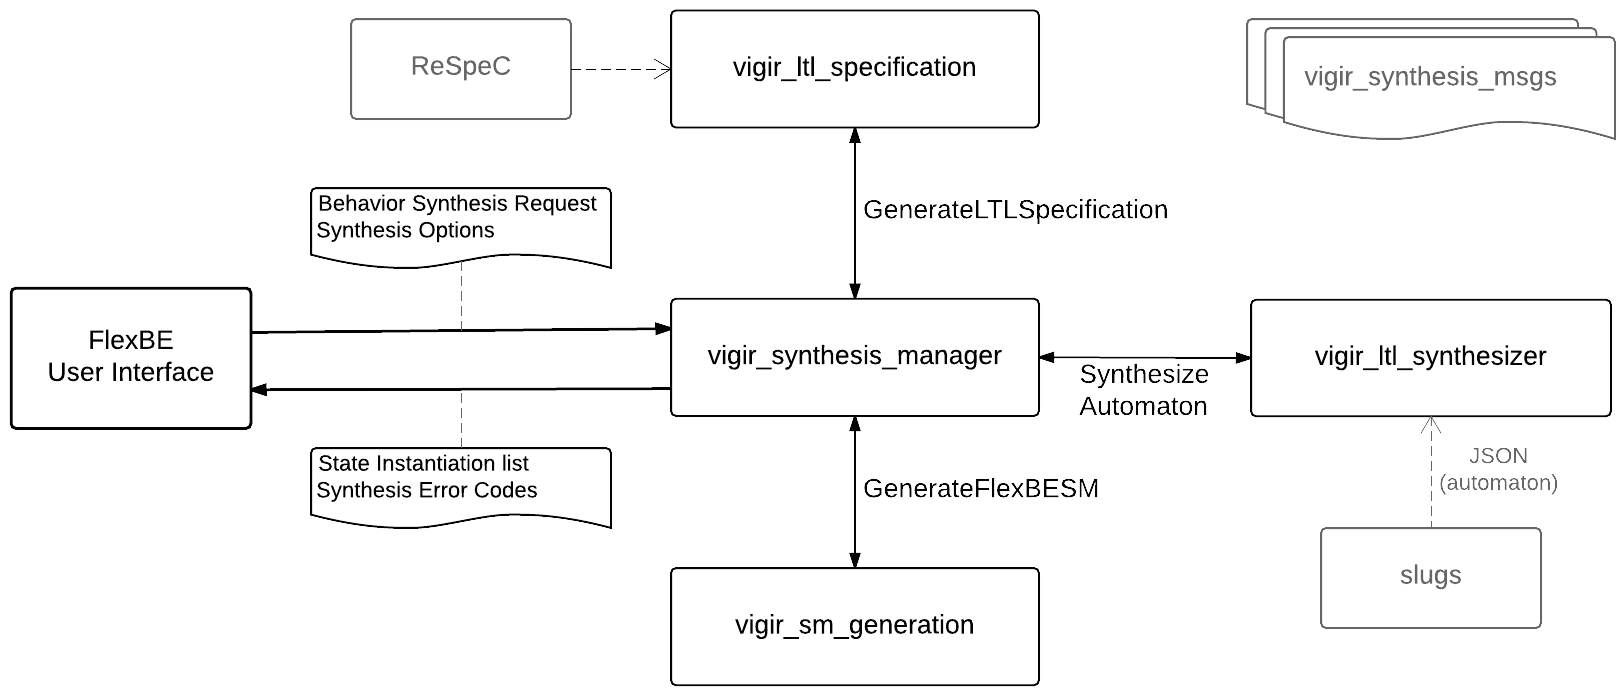
\includegraphics[width=0.99\columnwidth,clip]{./img/behavior_synthesis_packages.png}
\caption{
	Team ViGIR's ``Behavior Synthesis" ROS packages and the nominal workflow (clockwise, starting from the left).
}
\label{Fig:vigir_behavior_synthesis}
\end{figure}

The synthesis action server ($\mathtt{vigir\_synthesis\_manager}$) receives a request from the user via FlexBE's GUI.
Given the user's input (initial conditions and goals), the server first requests a full set of LTL formulas for Atlas from the $\mathtt{Generate LTL Specification}$ service ($\mathtt{vigir\_ltl\_specification}$ package).
The generation of the LTL formulas from Section \ref{S:ltl} is delegated to our ``Reactive Specification Construction kit" (ReSpeC),\footnote{\scriptsize{\url{https://github.com/team-vigir/ReSpeC}}}
 which is a Python framework with rudimentary ROS integration.

\begin{figure}[t]
\centering
\fbox{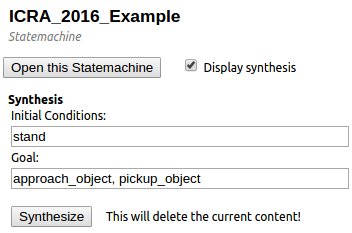
\includegraphics[width=0.90\columnwidth,clip]{./img/synthesis_menu_simple.png}}
\caption{Screenshot of the FlexBE Editor's synthesis menu.
}
\label{Fig:SynthesisMenuSimple}
\end{figure}

The $\mathtt{vigir\_ltl\_synthesizer}$ package acts as a wrapper for external synthesis tools (currently, \cite{SLUGS} is supported).
Given the generated LTL specification, the $\mathtt{Synthesize Automaton}$ service returns a finite-state automaton that is guaranteed to satisfy it, if one exists.
Finally, the server requests a $\mathtt{State Instantiation}$ message from the $\mathtt{Generate FlexBE SM}$ service ($\mathtt{vigir\_sm\_generation}$ package).
This message provides the FlexBE Editor with sufficient information to generate Python code, i.e., an executable state machine that instantiates the synthesized automaton.
The corresponding action, services, and messages are defined in the $\mathtt{vigir\_synthesis\_msgs}$ package.

%\begin{algorithm}[t]
The following excerpt\footnote{We have omitted some details for the sake of brevity and clarity of presentation. For example, most list elements are strings, e.g., \scriptsize{\texttt{"template\_id"}}.}
 is taken from the $\mathtt{State Instantiation}$ list message, which is the end product of the $\mathtt{vigir\_behavior\_synthesis}$ workflow (Fig. \ref{Fig:vigir_behavior_synthesis}).
Specifically, this excerpt corresponds to the primitive functionality $\mathtt{object\_template}$, which appears in Fig. \ref{Fig:stand_and_pick_sm}.

\begin{description}
\setlength{\itemindent}{-.4in}
	\item \scriptsize{\texttt{state\_path: /4\_object\_template}}
	\item \scriptsize{\texttt{state\_class: InputState}}
	\item \scriptsize{\texttt{parameter\_names: [request]}}
	\item \scriptsize{\texttt{parameter\_values: [InputState.SELECTED\_OBJECT\_ID]}}
	\item \scriptsize{\texttt{outcomes: [no\_connection, aborted, received, data\_error]}}
	\item \scriptsize{\texttt{transitions: [failed, failed, 6\_manipulate, failed]}}
	\item \scriptsize{\texttt{autonomy: [0, 0, 0, 0]}}
	\item \scriptsize{\texttt{userdata\_keys: [data]}}
	\item \scriptsize{\texttt{userdata\_remapping: [template\_id]}}
\end{description}

%\caption{Excerpt from $\mathtt{State Instantiation}$ message}
%\label{Alg:StateInstantiation}
%\end{algorithm}

% END
%
\section{Experimental Validation}\label{S:experiments}
% !TEX root = ../main.tex

\todo[inline, caption = {Synthesis time as a function to number of actions ?}]{Provide data on how computationally costly/cheap behavior synthesis is. Time vs number of actions?}

Team ViGIR did not employ high-level behavior synthesis during the DRC Finals.
However, we later carried out experimental demonstrations on \textsc{Atlas} in the lab.
Due to a hardware issue, \textsc{Atlas} could not locomote.
Thus, in addition to two experimental demonstrations, we present a simulation run carried out in Gazebo, using the same operator and onboard software.
We summarize these demonstrations below.
Please also refer to the accompanying video.

\subsection{Behavior Development using Synthesis}\label{S:SynthesisFromScratch}

In the first experimental demo, we show how a high-level behavior is specified and synthesized starting from scratch\footnote{The \textsc{ltl} specification and the synthesized automaton are available at: \scriptsize{\url{https://gist.github.com/spmaniato/c37fb12e874c73d986da}}}.
Once the state machine has been instantiated (Fig. \ref{Fig:stand_and_pick_sm}), it is ready for execution (Fig. \ref{Fig:stand_and_pick_gopro}).

\begin{figure}[t]
	\centering
	\begin{subfigure}[b]{0.99\columnwidth}
	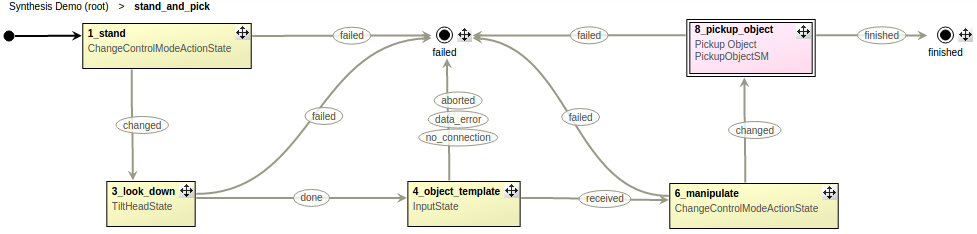
\includegraphics[width=0.99\columnwidth,clip]{./img/stand_and_pick_sm.png}
	\caption{
	The state machine above was synthesized for the task with $\mathcal{I} = \{ \mathtt{stand\_prep} \}$ and $\mathcal{G} = \{ \mathtt{look\_down}, \mathtt{pickup\_object} \}$.
	The capability $\mathtt{object\_template}$ requests an object template from the operator (Section \ref{S:TeamViGIR}).
	It is a precondition of $\mathtt{pickup\_object}$.
	}
	\label{Fig:stand_and_pick_sm}
	\end{subfigure}
	
	\vspace{4 pt}
	\begin{subfigure}[b]{0.95\columnwidth}
	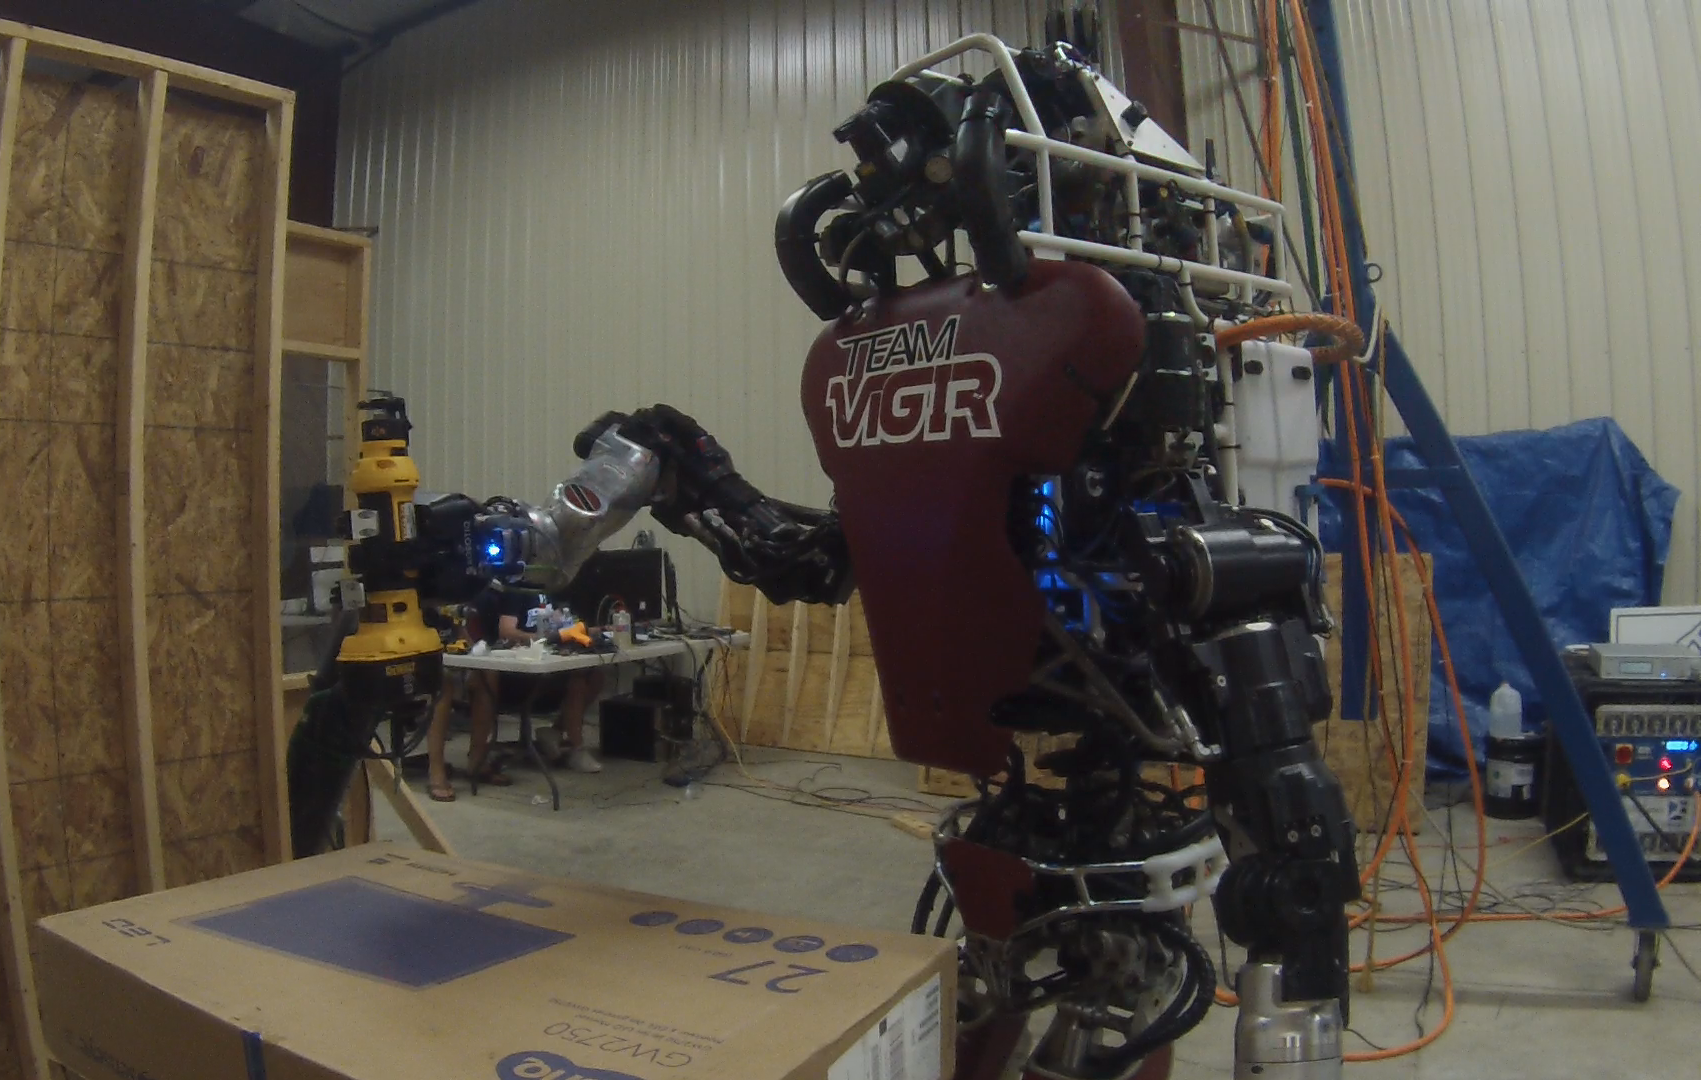
\includegraphics[width=0.99\columnwidth, clip]{./img/stand_and_pick_gopro.png}
	\caption{\textsc{Atlas} finishing execution of state $\mathtt{8\_pickup\_object}$.
	} 
	\label{Fig:stand_and_pick_gopro}
	\end{subfigure}
	\caption{
	Snapshots from the demo in Section \ref{S:SynthesisFromScratch}.
	}
	\label{Fig:stand_and_pick_demo}
\end{figure}

\subsection{Online Modifications using Synthesis}\label{S:RuntimeSynthesis}

For the second experimental demonstration, consider a scenario where the operator has designed a state machine that addresses a high-level task (either manually or via synthesis).
\textsc{Atlas} is then deployed and starts carrying out this task.
If, during execution, an \emph{unexpected} situation arises, the operator can use FlexBE's runtime modification capability (Fig. \ref{Fig:synthesis_runtime_demo}).
In this case, behavior execution is ``locked" at some state, i.e., this state is prevented from returning an outcome (Fig. \ref{Fig:runtime1}). 
Then, the operator specifies a new high-level behavior meant to address the unexpected situation.
Once this new state machine is instantiated (Fig. \ref{Fig:runtime2}), it is connected to the previous one (Fig. \ref{Fig:runtime1}), and execution resumes.

\begin{figure}[t]
	\centering
	\begin{subfigure}[b]{0.99\columnwidth}
	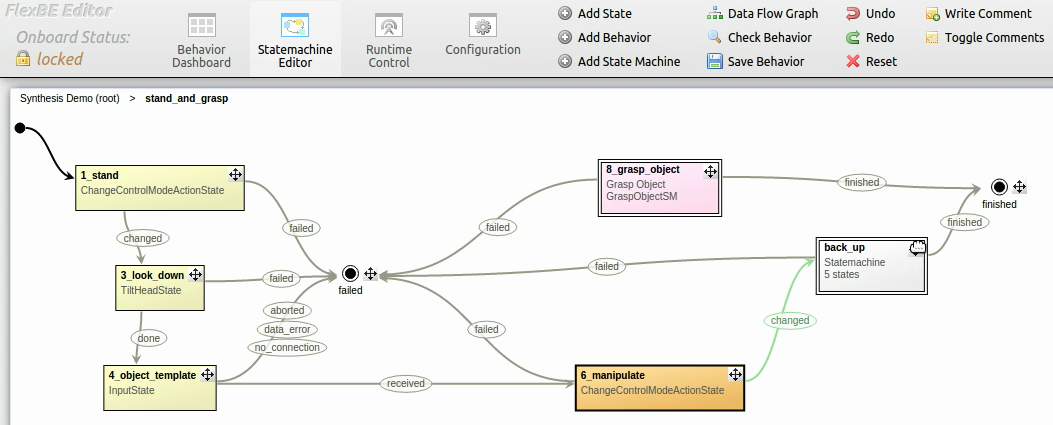
\includegraphics[width=0.99\columnwidth, clip]{./img/synthesis_runtime_connect_sm.png}
	\caption{The operator ``locks" the initial state machine at the state $\mathtt{6\_manipulate}$ (indicated by the orange color), which is allowed to be executed.
	Then, a new state machine, $\mathtt{back\_up}$, is synthesized with $\mathtt{manipulate}$ as the initial condition.
	The transition from $\mathtt{6\_manipulate}$ is then moved from $\mathtt{8\_grasp\_object}$ to $\mathtt{back\_up}$.
	} 
	\label{Fig:runtime1}
	\end{subfigure}
	
	\vspace{4 pt}
	\begin{subfigure}[b]{0.99\columnwidth}
	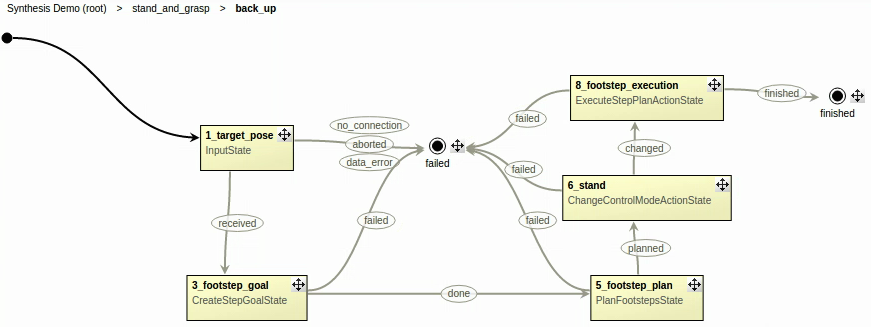
\includegraphics[width=0.99\columnwidth, clip]{./img/synthesis_runtime_synthesized_sm.png}
	\caption{The new state machine, $\mathtt{back\_up}$, was synthesized for the task with $\mathcal{I} = \{ \mathtt{manipulate} \}$ and $\mathcal{G} = \{ \mathtt{footstep\_execution} \}$.
	} 
	\label{Fig:runtime2}
	\end{subfigure}
	\caption{
	FlexBE Editor snapshots from the demo in Section \ref{S:RuntimeSynthesis}.
%	During execution of the $\mathtt{stand\_and\_grasp}$ state machine, an unexpected situation arises.
	In response to some unexpected event, the operator synthesized a state machine that has \textsc{Atlas} back away (\ref{Fig:runtime2}).
	}
	\label{Fig:synthesis_runtime_demo}
\end{figure}

%\subsection{Infinite execution or Footstep stuff (simulation)}
%
%For example, ``From stand-prep, walk to object, pick it up, (go to stand-manipulate), carry object, release, and repeat"

% END
%
\section{Conclusions and Future Work}\label{S:conclusion}
% !TEX root = ../main.tex

We presented an end-to-end approach to mission planning for complex robotic systems.
We combined a task, specified by a non-expert user, with a discrete abstraction of the system, defined \emph{a priori}, to automatically generate a formal specification.
We then synthesized a provably correct mission plan that achieves the task's goals or reacts to any failures in the low-level system components.
Finally, we automatically generated a software implementation of the mission plan in the form of an executable state machine.
We implemented our approach as a collection of ROS packages and experimentally validated it on an Atlas humanoid robot running the software that Team ViGIR developed for the DRC.

It is important to point out the trade-off between expressivity and automation.
On the one hand, an expert user can manually write a very expressive and customized formal specification.
On the other hand, the generation of the formal specification can be automated, as we do here, but possibly at the expense of expressivity (e.g., due to hard-coded design choices.)
However, there is no research barrier to recovering expressivity; the formal language supports it.
Thus, we plan on extending our user interface in immediate future work.

The discrete abstraction and formal specification paradigm that we presented in this paper constitute the first steps towards achieving graceful degradation.
In other words, we hinted at the question, ``What formal guarantees can we offer when the execution of robot capabilities can result in failure?"
We plan on further exploring this research direction.

We are also interested in automating the construction of the discrete abstraction, which includes action preconditions, outcomes, etc.
Currently, the system designer defines it (once per system).
We believe that, by formally specifying the capabilities and constraints of individual system components, we will be able to automatically generate the discrete abstraction.
Finally, we will be demonstrating our approach on a number of different robotic systems in the near future.

%END
%
\section*{Acknowledgments}
The authors thank all other members of Team ViGIR and especially Alberto Romay, Stefan Kohlbrecher, and Prof. Oskar von Stryk from Technische Universit\"{a}t Darmstadt.
%
% ---- Bibliography ----
%
\bibliographystyle{ieeetran}
\bibliography{behavior_synthesis}
%
\end{document}
